\section{Theory}
\vspace{-0.5cm}
\singlespacing

\textit{Torque} is the measure of force needed to cause an object to rotate. Torque can be calculated by multiplying the force applied to an object, the radius of that force from the object's pivot point, and the angle between the component of the force that is perpendicular to the pivot axis. This relationship between the angle of the force applied, and an object's pivot point can be represented using the following equation:

\begin{align*}
	T = \left| r \right | \left | F \right| \sin \theta 
\end{align*}

Since gravity is a force that acts on all parts of an object, it applies torque at multiple points at the same time. Instead of calculating the torque caused by gravity at multiple positions on an object, a single position, the object's \textit{center of mass}, is used. Objects with a uniform distribution of mass, typically symmetrical with no varying mass, usually have their center of mass right at the center as shown below:

\begin{figure}[H]
	\begin{center}
		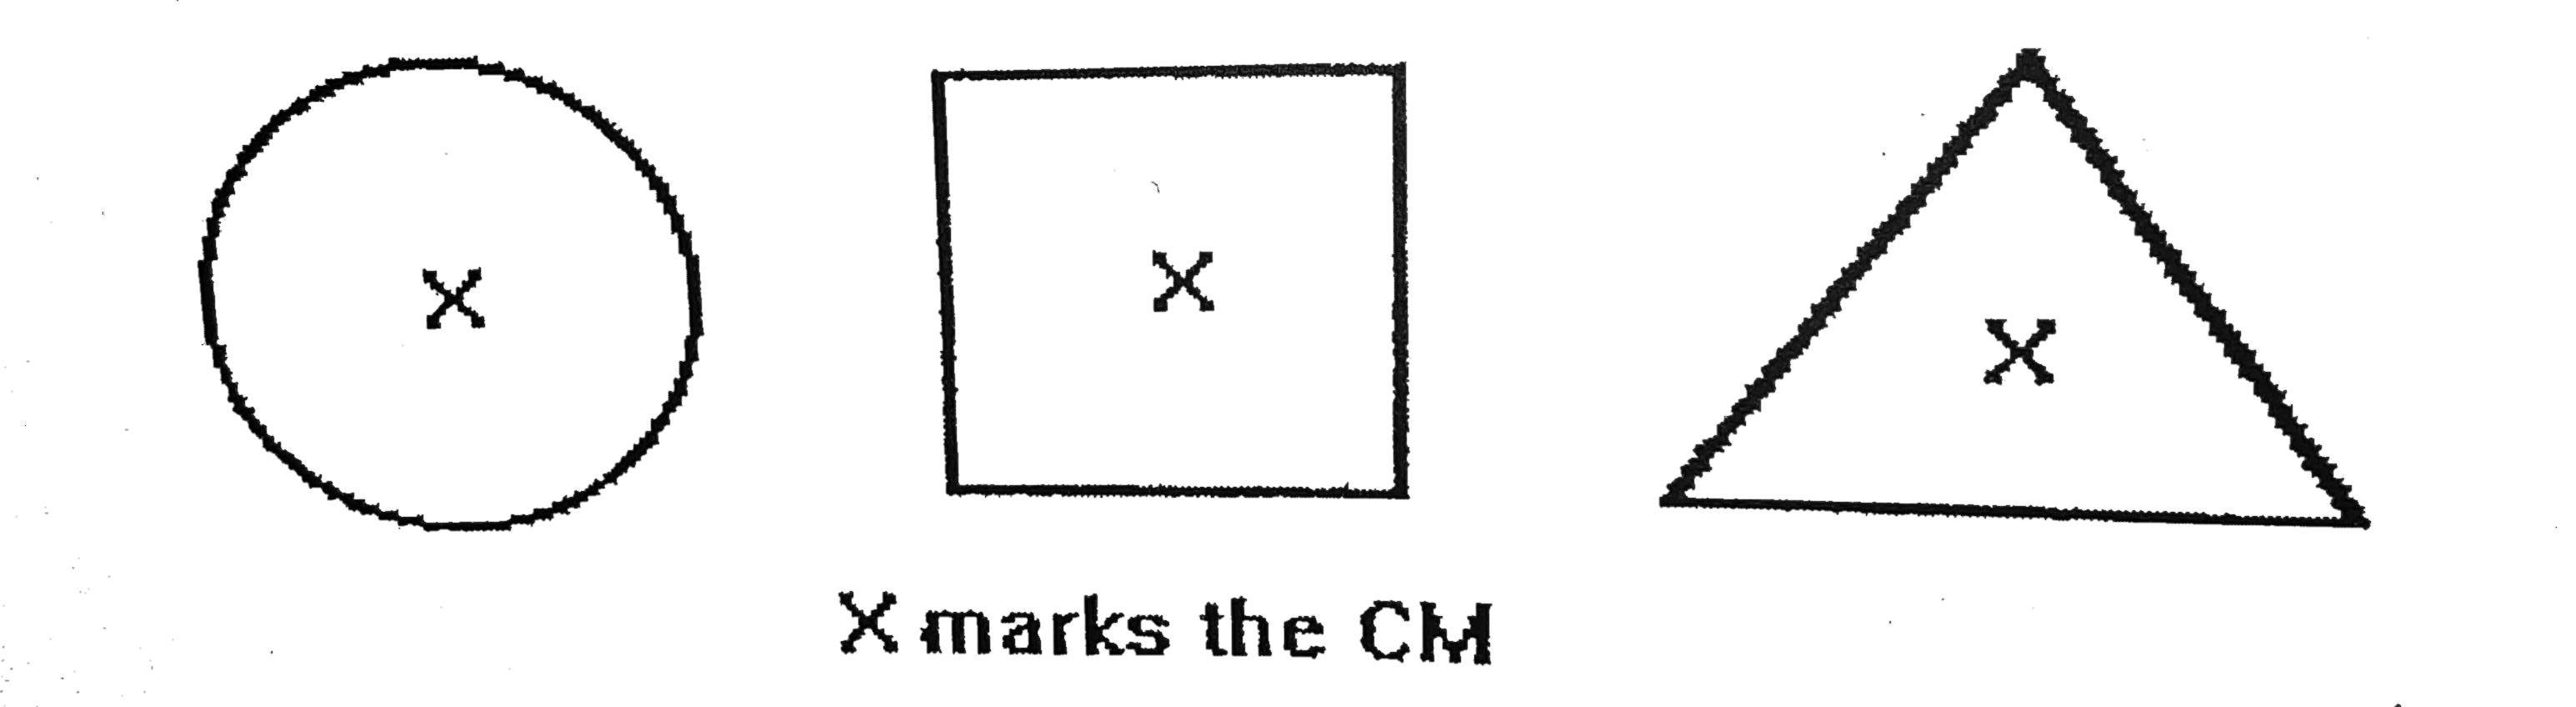
\includegraphics[width=0.55\textwidth]{comEx.jpg}
	\end{center}
	\caption{Symmetrical objects usually have their center of mass...at the center.}\label{fig:comEx}
\end{figure}

An object's center of mass can be calculated using the following equation:

\begin{align*}
	x_\text{com} &= \frac{m_1x_1 + m_2x_2 + ...}{M_T} \\ \\
x_\text{com} &: \text{center of mass} \\
	m_1 &: \text{mass of object 1} \\
	m_2 &: \text{mass of object 2} \\
	x_1 &: \text{position of object 1} \\
	x_2 &: \text{position of object 2} \\
	M_T &: \text{total mass of system}
\end{align*}

\newpage
